
\subsection{New vision of Data Integration}
Let us assume the following medical scenario in which users are able to retrieve and integrate data concerning (i) \textit{patients that were infected by a disease;}
(ii) \textit{regions most affected by a disease in specific region}; (iii)
\textit{patients' personal information}; and (iv) \textit{patients' DNA
information}.

The figure~\ref{fig:scenario} illustrates our vision of data integration. Data is delivered as \textit{data services} deployed in a multi-cloud context. Each \textit{data service} and cloud export their SLA specifying the level of services, the available services and their cost, and the access conditions the user can expect. Therefore, given a user query, her integration quality requirements and her cloud subscription, it is rewritten in terms of cloud services (\textit{data services} and \textit{data processing services}) composition that fulfill the integration requirements and deliver the expected results to the user.

\begin{figure}[h!]
\center
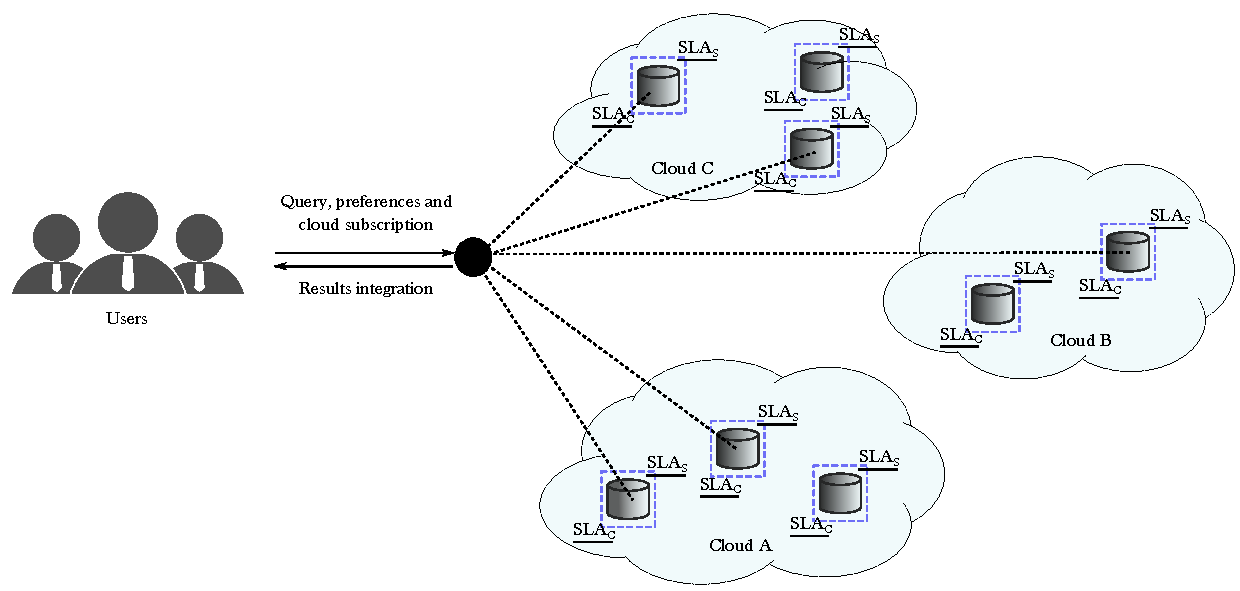
\includegraphics[scale=0.57]{scenario.pdf}
\caption{Data integration scenario}\label{fig:scenario}
\end{figure}

Taking into consideration the medical scenario, Doctor \textit{Marcel}'s research is interested in the type of people suffering of \textit{flu} in the Europe. He has at his disposal a set of cloud services delivered by different clouds. To reach his needs, he wants to query the personal information and DNA information from patients that were infected by \textit{flu}, using services with availability higher than 98\%, price per call less than 0.2\$ and integration total cost less than 5\$. This new context brings challenges to data integration, such as:
\begin{itemize}
\item \textbf{Performance}. In the multi-cloud, the amount of available services is high. Consequently, the processing time necessary to produce service compositions (given the high number of services) and to execute them is also high.
\item \textbf{Economic model}. Even with the possibility of having an unlimited access to resources, the user is limited to the resources she has contracted and to the budget she is ready to pay for. Thus, it is necessary to produce the rewritings satisfying the user integration requirements. 
\item \textbf{Quality}. Part of the rewritings produced to the user query does not satisfy her quality requirements concerning privacy, data provenance, cost, among others. Producing these rewritings implies increasing time processing and cost. 
\item \textbf{Matching problem}. While producing the rewritings, it is necessary to match the user requirements with the different SLAs exported by the cloud providers and cloud services. In the multi-cloud, cloud providers and cloud services export SLAs with different semantics and structure that makes the matching SLA and user requirement challenging. In addition, it also deals with incompatibilities of SLAs.
\item \textbf{Reuse}. Rewriting and executing the user query is computationally costly in terms of processing time and economic cost. Thus, it is necessary to propose a manner of reusing previous integration in order to save time and money, but also meeting the user expectations.
\end{itemize}

\subsection{Approach}
Thus, motivated by these challenges, a SLA guided data integration approach can be divided in four steps. Given a user query, a set of user preferences associated to it, cloud providers and cloud services:
\\
\textbf{\underline{SLA derivation}}. This step creates an \textsl{integrated
SLA} that includes a set of measures corresponding to the user preferences. The \textsl{integrated SLA} guides the query evaluation, and the way results are computed and delivered. \\
\textbf{\underline{Filtering data services}}. The \textsl{integrated SLA} is used (i)
to filter previous SLA derived for a similar request in order to reuse previous results; or (ii) to filter possible data services that can be used for answering the query. \\
\textbf{\underline{Query rewriting}}. Given a set of data services that can
potentially provide data for integrating the query result, a set of service compositions is generated according to the \textsl{integrated SLA} and the agreed SLA of each data service. \\
\textbf{\underline{Integrating a query result}}. The service compositions are executed
in one or several clouds where the user has a subscription. The execution cost of service compositions must fulfill the \textsl{integrated SLA} (that expresses user requirements). Here, the clouds resources needed to execute the composition and how to use them is decided taking in consideration the economic cost determined by the data to be transferred, the number of external calls to services, data storage and delivery cost.

Although \textit{the SLA derivation} is the big challenge while dealing with
SLAs and particularly for adding quality dimensions to data integration, the
focus in this paper is our query rewriting algorithm which deals with user
preferences and SLAs exported by different cloud providers and data services.
Here, we are assuming that there is a mechanism responsible to extract the
services' quality aspects from SLA, and to provide this information as input to
the algorithm. The figure~\ref{fig:cloudsla} illustrates the structure of SLA
and its measures that are considered in the approach we will detail in the next
section.   

\subsection{SLA model}

\subsection{Query rewriting algorithm}

\begin{figure}[h!]
\center
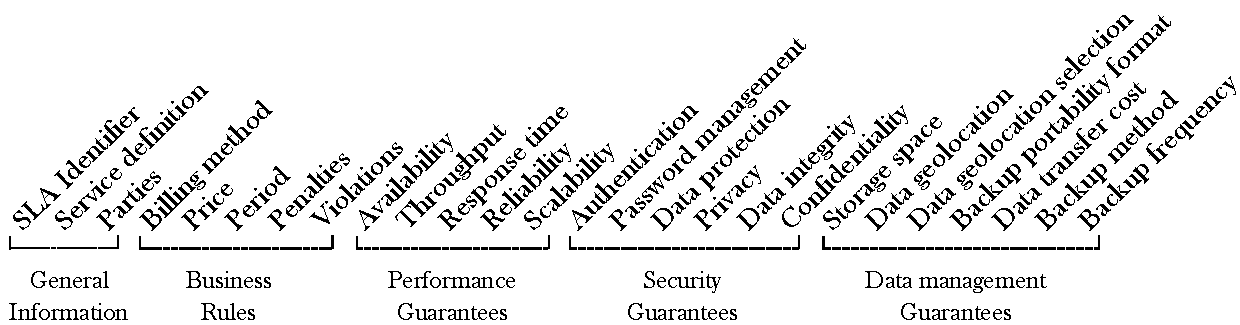
\includegraphics[scale=0.57]{Cloud_SLA.pdf}
\caption{Cloud SLA}\label{fig:cloudsla}
\end{figure}